\section{Data}\label{sec:Data}
Most of the available literature regarding the impact of ETF ownership on stock's volatility and liquidity uses a specialized dataset that was unfortunately not available for this paper, namely the Thomson Reuters Mutual Fund Ownership Database also known as S12. Completeness is theoretically guaranteed in this dataset since its direct source is the filings that all investment companies\footnote{A note by Wharton Research Data Services at the University of Pennsylvania lists the various types of investment companies reporting their holdings : ``banks, insurance companies, parents of mutual funds, pension funds, university endomwents [as well as][...] professional investment advisors''. Together, because of the form they report current assets held, they are called \textit{13f institutions} and file with the regulator at least quarterly.} have to report quarterly to the U.S. Securities and Exchange Commission (SEC). Whereas access to the Institutional Holdings (aggregated at the management companies' level), also known as S34, were available through WRDS at the University of Pennsyvania, they lacked granularity since most of if not all the major ETFs (according to the amount of funds held) are issued by a limited number of investment management companies. Nevertheless, Thomson Reuters data regarding the fund ownership of stocks can be found alternatively on their \textit{Eikon} platform and the systematic lookup is implemented through an open application programmation interface (API) for which libraries have been written in common programming languages. Nevertheless, the origin of fund holdings data is less clear as I cannot ascertain that they come from S12 nor that they have not been modified before integration in \textit{Eikon}\footnote{As of the date of redaction of this section, transition is ongoing towards a rebranding of the mentioned products, after the sale of the data unit of Thomson Reuters to Refinitiv.}.

The availability of ETF ownership is the critical variables when it comes to put time boundaries to the analysis : there are ETF holdings before 1999, whereas the Thomson Reuters Mutual Fund Ownership database starts around 1980 and would therefore theoretically allow to track the first ETFs active in the US ever, back in the early 1990s. Nevertheless, the aggregate value invested in those funds was almost insignificant during most of the decade and therefore I choose to collect month-end observations from January 1999 to December 2018, that is, over 240 months. Further restrictions due to lags will limit the effective length of the panel.  
\subsection{Exchange-Traded Funds characteristics}
One of the most extensive sources of basic ETF data may be the items under share code \texttt{73} in the dataset maintained by the Center for Research in Security Prices (CRSP) at the University of Chicago, with access again granted through WRDS. Since the first Exchange-Traded Fund's inception in 1990 in Canada, they refer 2893 funds in this category, with the important restriction that CRSP only tracks securities in the United States. Without any restriction on the country of incorporation, Thomson Reuters exhibits 4085 active ETFs and it is not possible to get the sample of discontinued ETFs; on the other hand, the active sample seems to be a substantial share of all ETFs currently live worldwide.

In general, index-tracking ETFs\footnote{The context of this analysis still can be summarized as a gross distinction between mutual funds (actively managed, open-end funds without intraday liquidity and priced at their Net Asset Value at market close), index funds which are their passive counterpart (e.g. the iconic Vanguard 500 Index Fund with its beta of 1.00 to the S\&P 500 equity index) and the ETFs that are open-end, index-tracking funds with a continuous arbitrage mechanism enabled by issuing their indicative intraday NAV every 15 seconds throughout the day. This polarized landscape has been changing during the last decade though : preliminary results (\textcite{Easley2018}) show that the share of ETFs explicitly labelled as active portfolios has been increasing (1.8\% of assets under management in US equity ETF as of 2017, \textcite{Ben-David2017}) while somewhat mixed performance relative to their benchmarks have made mutual funds less reliant on their managers' skills} may engage in three different implementations of index-tracking:
\begin{description}
\item[Full (or \textit{physical}) replication] The securities in the index portfolio are all held by the ETF in the actual proportions used to compute the index. We could say that this product is fully collateralized. 
\item[Optimized replication] The ETF generally uses a proprietary algorithm to tilt its holdings towards the securities with the most contribution to the index volatility. Thus smaller securities encompassed by the index are neglected, in whole or in part.
  \item[Swap-based replication] The ETF does not hold the ``physical'' securities but enters into derivatives such as a total return swap agreements which replicate the index performance including cash flows such as dividends. ETF shares creations and redemptions are therefore made in cash. Swap-based ETFs indirectly allow investors to access swaps while they - especially individuals - would not be able to enter such contracts with a bank on their own, but those products also expose them to the counterparty risk in exchage for tax advantages (i.e. income treated as capital gain). 
\end{description}
While swap-based replication for instance allows leveraged and inverse ETFs, thefact those products do not actually trade the underlying securities prevents a demand shock happening on themselves from subsequently influencing the volatilityand liquidity of stocks. Since they constitute a minority of the broad ETF market in terms of value, especially in the United States, they are not kept in the sample of interest. Hence, there are 1798 full-replication, 1497 (explicitly) optimized-replication ETFs and 29 more exhibiting \textit{Other}. Their documentation shows it means either an optimization regarding a specific sector or a mix between a majority of physical shares and derivatives in addition. It is relatively more worrying to acknowledge the 277 funds for which the value of the \texttt{Index replication method} variable is missing. At least a part among them may be actually swap- or option-based and therefore hold no physical asset -- in which case, they could have been excluded from the sample of 3324 remaining ETFs. \autoref{fig:Data:Entities} tracks the number of live entities (funds) month by month in the U.S. sample, since the inception of the first one (actually, the SPY) and whenever the information about inception/deletion is available; \autoref{tab:ETFCharacteristics} shows the unequal availability of ETF characteristics, which may limit the relevance of qualitative descriptions. 

\begin{figure}
    \centering
    \caption{Number of ETFs included over the sample period}
    \label{fig:Data:Entities}
    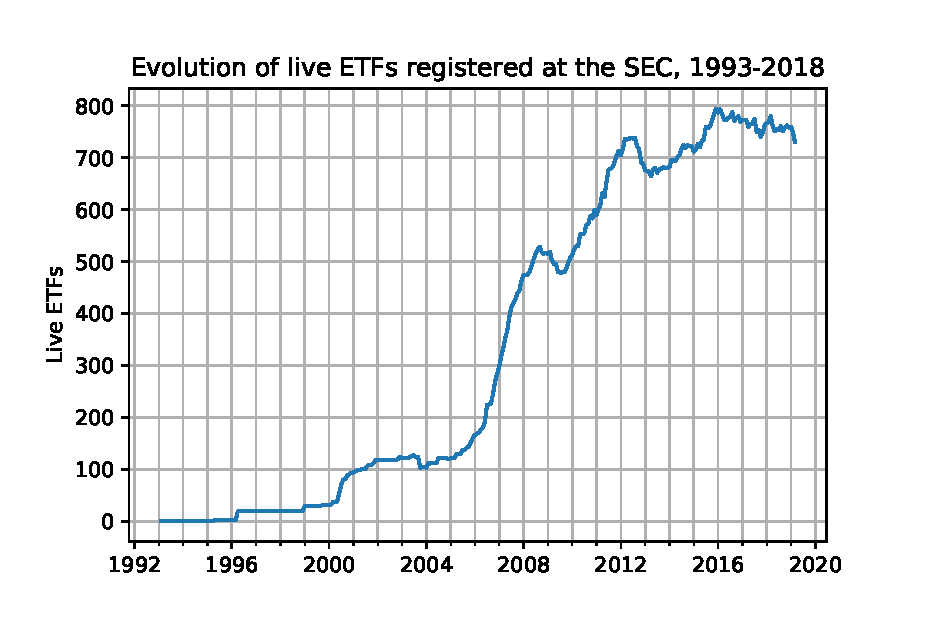
\includegraphics[width = \textwidth, height = 0.3\paperheight, keepaspectratio]{./Slides/LiveETF_Eikon}\\
    {\footnotesize Computation by the author; data from \emph{Eikon} fund screener, only physical- and optimized-replication ETFs listed in the U.S.}
\end{figure}

{\linespread{1.0}
\begin{table}[htbp]
\centering
  \caption{Summary of the variables' coverage in the ETF Characteristics table}
  \label{tab:ETFCharacteristics}
  \begin{tabular}{lr}
    \toprule
    Data columns & (total 20 columns)\\
    \midrule
    Lipper\_RIC & 3601 non-null object\\
    CUSIP & 1814 non-null object\\
    ISIN\_Code & 3577 non-null object\\
    Asset\_Name & 3601 non-null object\\
    Asset\_Full\_Name & 1990 non-null object\\
    SEC\_Inception\_Date & 1378 non-null datetime64[ns]\\
    Fund\_Management\_Company\_Long\_Name & 3601 non-null object\\
    Closed\_Date & 0 non-null float64\\
    Exchange\_Traded\_Fund(ETF) & 3601 non-null int64\\
    ETF\_Ticker & 2509 non-null object\\
    Asset\_Status & 3601 non-null object\\
    UCITS & 736 non-null float64\\
    Legal\_Structure & 2221 non-null object\\
    Index\_Tracking & 3333 non-null float64\\
    Index\_Replication\_Method & 3324 non-null object\\
    Investment\_Objective & 3600 non-null object\\
    Style\_Matrix & 1223 non-null object\\
    Broad-Based\_Index & 1376 non-null object\\
    Peer\_Index & 1369 non-null object\\
    \bottomrule
  \end{tabular}
  {\itshape
  \begin{tabular}{rr}
  Type: & <class 'pandas.core.frame.DataFrame'>\\
  RangeIndex: & 3601 entries, 0 to 3600\\
  dtypes: & datetime64[ns](1), float64(3), int64(2), object(14)\\
  Memory usage: & 562.7+ KB
  \end{tabular}}
\end{table}
}


\subsection{Common stocks' fund ownership}
The sample of live U.S.-traded stocks provided through the Screener function in Eikon is the basis for this analysis; it does not only include companies that are headquartered in the United States but also foreign (from the U.S. point of view) ones with a listing on a U.S. stock exchange. Overall, the sample contains 4978 active companies (as of March 4, 2019) with no conditioning on size, lifetime nor stock price; out of them, 4426 are U.S. companies and the remainder is split across 48 other countries, with almost 30\% of them being located in China.

Fund ownership is available through the variable \texttt{TR.FundAdjShrsHeld}, meaning \textit{the number of shares of a given stock held by a given fund, adjusted for corporate actions (e.g. stock splits)}. For a stock at a given date, a query through the Thomson Reuters Eikon API allows to retrieve the whole fund ownership at once (ignoring the reporting issues\dots), with the fund ID, category and an essential information : the date of holdings reporting, which is a metadata of the shares held value. Enquiries in the database have shown that ETF holdings are generally up to date, whereas a larger share of other funds exhibit a reporting delay, i.e. a reporting date earlier than the query date. Indeed, in order not to introduce erroneous data, no spurious extrapolation (from the latest reported date to the query date) is decided, except if both dates lie in the same momth of the same year. Once they are grouped by month of report, only holdings of ETFs are kept, they are summed at the stock level and finally divided by the number of shares outstanding at month end (adjusted for corporate actions) to obtain the relative ETF ownership. Some outliers above or close to 100\% ownership have been identified when specific companies went under the Chapter 11 protection of the US Bankruptcy Code and the fund amounts of shares held were not immediately updated for the equity being destroyed. Whenever this case occurred, the \textit{de facto} invalid observations have been dropped. The final sample for U.S. stocks includes $712445$ non-null observations.
\subsection{Common stocks' market and accounting data}
The Eikon API also provides an extensive access to time series of market data, of which daily close price, traded volume in terms of shares and -- in order to compute the \textcite{Amihud2002} illiquidity ratio, a control variable -- the volume-weighted average price (VWAP). Cross-sectional queries, similar to those regarding fund ownership, allowed to retrieve the remaining control variables, respectively the input necessary to compute them. Availability differs for every variable in the panel, which limits the number of observations actually used; by its very nature of gathering stocks that have entered the sample at different times over twenty years, the panel is heavily unbalanced, which does not prevent the statistical analysis to hold as long as the availability of data is not correlated with variables of interest.

As it is obvious from \autoref{tab:AssetCategories} which sorts the frequencies of entities across subsamples and overall, the vast majority of securities identified through a unique Reuters Identifier Code (RIC) are ordinary shares, i.e. common equity stock. The first two rows gather more than 97.5\% of the sample and the remainder is scattered across multiple categories. The three next most frequent categories are close to stock (preference share is a synonym for preferred stock and American depository receipt, the latter being a proxy for a foreign (non-U.S.) stock issued by a U.S.-based bank) or to trusts (the ``Unit'' category). The numerous marginal types are either country-specific investment vehicles or clearly outliers for which one can suspect a classification error (bonds, exchange-trade products. The general statement taught through this category breakdown is that the securities from this global sample do not exclusively belong to common stock, although an overwhelming majority does. Still, the total value of those alternative vehicles held through ETFs is likely not a significant share since they focus their equity investments on large-cap and liquid equity. A possible robustness check would be to further restrict the following analysis to actual ordinary equity shares. 

%\begin{center}
 % \textsc{TBD : Summary of availability of data across time, size deciles (?)}
  %\textsc{TBD : Table and figure for percentage of market cap across percentiles(above\/below median, in the S\&P 500/Russell 3000 fashion of \textcite{Ben-David2018})}
%\end{center}

{\linespread{1.0}
\begin{table}
  \centering
  \caption{U.S. and International broad samples of underlying securities: categories of instruments}
  \label{tab:AssetCategories}
  \begin{tabular}{lrrr}
\toprule
Asset Category Description  &  International &    US &    All \\
\midrule
Ordinary Share                  &          15225 &  4634 &  19859 \\
Fully Paid Ordinary Share       &           1030 &     5 &   1035 \\
Unit                            &             57 &   114 &    171 \\
American Depository Receipt     &              0 &   127 &    127 \\
Preference Share                &            105 &     0 &    105 \\
Global Depository Receipt       &             13 &     0 &     13 \\
Participation Share             &             13 &     0 &     13 \\
Depository Receipt              &              7 &     4 &     11 \\
Closed-End Fund                 &              6 &     3 &      9 \\
Dutch Certificate               &              7 &     0 &      7 \\
Brazilian Unit                  &              5 &     0 &      5 \\
Preferred Share                 &              2 &     2 &      4 \\
Stapled Security                &              3 &     1 &      4 \\
Bond                            &              2 &     1 &      3 \\
Swedish Depository Receipt      &              3 &     0 &      3 \\
Brazilian Depository Receipt    &              2 &     0 &      2 \\
Genussschein                    &              2 &     0 &      2 \\
Savings Share                   &              2 &     0 &      2 \\
Convertible Preference Share    &              0 &     1 &      1 \\
Exchange-Traded Commodity       &              1 &     0 &      1 \\
Exchange-Traded Note            &              1 &     0 &      1 \\
Non-Cumulative Preference Share &              1 &     0 &      1 \\
No available information        &              9 &    20 &     29 \\
\midrule
All                             &          16496 &  4912 &  21408 \\
\bottomrule
\end{tabular}

\end{table}
}

